\documentclass[12pt]{article}

\usepackage{pgfplots}
\usepackage{amstext,amsfonts,amssymb,amscd,amsbsy,amsmath,graphicx}
\usepackage{amstext,amsfonts,amssymb,amscd,amsbsy,amsmath,graphicx,adjustbox}
\pagestyle{empty}
%\parindent = 0in
\usepackage{parskip}%this removes paragraph indents #emilyforthewin#blessed

\pagestyle{empty}
%\parindent = 0in
\usepackage{parskip}%this removes paragraph indents #emilyforthewin#blessed
\usepackage[margin=0.4in]{geometry}

\begin{document}
\begin{center}
Math 101 Review: Exam 1
\end{center}
\begin{enumerate}
    \item Consider the following table: 
\begin{center}
\begin{tabular}{c || c | c | c | c}
$x$ & -3 & 1 & 3 & $\star$ \\\hline
$f(x)$ & -3 & 6 & 7 & 3
\end{tabular}


\end{center}
Give a value for $\star$ so that $f(x)$ is a function. What values are we not allowed to have for $\star$?
\vspace{1in}

\item Suppose the points $(2,4)$ and $(6,16)$ are on the function $f(x)$. Find $f(x)$ assuming it is linear.

\vspace{1.in}

\item Determine whether the functions in the following tables could be linear.  If a function is linear, find a formula for it.  If a function is not linear, explain how you know. 

\begin{itemize}
\item[(a)] \hspace{1px} \vspace{-0.25in}

\begin{center}
\begin{tabular}{c || c | c | c | c}
$x$ & -3 & 0 & 6 & 18 \\\hline
$f(x)$ & -17 & -16 & -14 & 0
\end{tabular}
\end{center}
\vspace{2.5in}
\item[(b)] \hspace{1px}\vspace{-0.25in}

\begin{center}
\begin{tabular}{c || c | c | c | c}
$x$ & -2 & -1 & 0 & 2 \\\hline
$g(x)$ & -1 & -3 & -9 & -81
\end{tabular}
\end{center}

\end{itemize}

\newpage


%\item Suppose that the height of water in a cylidrical tank increases by 0.25 feet per hour.
%
%\begin{itemize}
%\item[(a)] Find a function $H$, the height of the water in the tank, as a function of $t$, the number of hours that has elapsed.
%\vspace{1in}
%
%\item[(b)] The volume of water in the tank when the height is $h$ feet is $V(h)=25\pi h$ cubic feet. Using (a), find a formula for $V=f(t)$, the volume of water in the tank after $t$ hours. 
%\vspace{1in}
%\end{itemize}


\item Last winter, Anne measured the height of snow on her sidewalk during a blizzard. She defined the function $s(t)$, which gives the height of snow in inches $t$ hours after she started measuring.

\begin{figure}[h!]
\begin{center}
\begin{tikzpicture}[yscale=.75]
\draw [->] (-0.5,0) -- (4.5,0) node [right] {$t$};
\draw [->] (0,-0.5) -- (0,6.5) node [above] {$s(t)$};
\foreach \x in {1,2,3,4}
	\draw (\x,-.2) -- (\x,.2) node [at start, below] {\footnotesize\x};
\foreach \y in {2,4,6}
	\draw (-.2,\y) -- (.2,\y) node [at start, left] {\footnotesize\y};
\foreach \y in {1,3,5}
	\draw (-.2,\y) -- (0.2,\y);
\draw [very thick, domain=0:2, smooth, variable=\x] plot ({\x},{2*\x+2});
\draw [->, very thick, domain=2:5, smooth, variable=\x] plot ({\x},{0.5*\x-1});
\draw [fill=black] (0,2) circle [radius=3pt] (2,0) circle [radius=3pt] (4,1) circle [radius=3pt];
\draw [fill=white] (2,6) circle [radius=3pt];
\end{tikzpicture}
\end{center}
\end{figure}
Using the graph, write a piecewise function for $s(t)$ (show all of your work):

\[\scalebox{1.5}{$s(t)=\begin{cases}
\underline{\hspace{1.5in}}\qquad&\text{for }\underline{\hspace{.3in}} \leq t < \underline{\hspace{.3in}} \\[3ex]
\underline{\hspace{1.5in}}\qquad&\text{for } t \geq \underline{\hspace{.3in}} 
\end{cases}$}\]

\vspace{1 in}

\item Find the average rate of change of $f(x)=\frac{x}{x^2+1}$ on the interval $[-1,1]$. If you have a graphing device, sketch the function along with the line between $(-1,f(-1))$ and $(1,f(1))$. What do you notice about the lines slope? 
\vspace{2in}


\newpage

\item For the graphs and tables below, use the definition of a function to explain whether or not each one represents a function.\\

\begin{enumerate}
    \item \begin{tabular}{|c||c|c|c|c|c|}
\hline
$x$ & 8 & 9 & 12 & 13 & 15 \\ \hline
$y$ & -2 & 3 & 4 & -2 & 7\\ \hline
\end{tabular}

\vspace{.5in}


\item\begin{tikzpicture}[scale=.45]
\draw [<->] (-5,0) -- (5,0) node [right] {$x$};
\draw [<->] (0,-5) -- (0,5) node [above] {$y$};
\foreach \x in {-4,-2,2,4}
	\draw (\x,-.2) -- (\x,.2) node [above] {\footnotesize\x};
\foreach \y in {-4,-2,2,4}
	\draw (-.2,\y) -- (.2,\y) node [right] {\footnotesize\y};
\draw [very thick, domain=-4:-2, smooth, variable=\x] plot ({\x},{-3});
\draw [very thick, domain=-2:0, smooth, variable=\x] plot ({\x},{-1});
\draw [very thick, domain=0:2, smooth, variable=\x] plot ({\x},{1});
\draw [very thick, domain=2:4, smooth, variable=\x] plot ({\x},{3});
\draw [fill=black] (-4,-3) circle [radius=3pt] (-2,-1) circle [radius=3pt] (0,1) circle [radius=3pt] (2,3) circle [radius=3pt];
\draw [fill=white] (-2,-3) circle [radius=3pt] (0,-1) circle [radius=3pt] (2,1) circle [radius=3pt] (4,3) circle [radius=3pt];
\end{tikzpicture}

\vspace{.5in}

\item \renewcommand\arraystretch{1.2}
\begin{tabular}{|c||c|c|c|c|c|}
\hline
$x$ & 7 & 6 & 7 & 4 & 2 \\ \hline
$y$ & 5 & -4 & 2 & 3 & 9 \\ \hline
\end{tabular}

\vspace{.5in}


\item 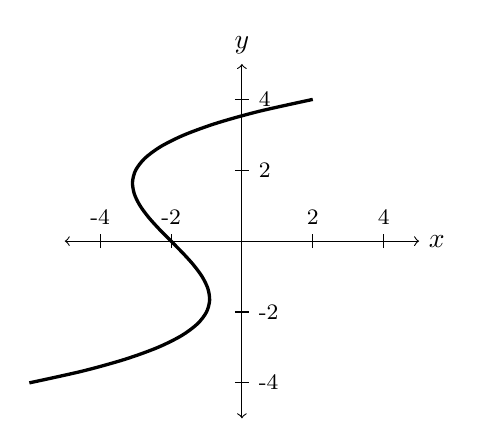
\begin{tikzpicture}[scale=.45]
\draw [<->] (-5,0) -- (5,0) node [right] {$x$};
\draw [<->] (0,-5) -- (0,5) node [above] {$y$};
\foreach \x in {-4,-2,2,4}
	\draw (\x,-.2) -- (\x,.2) node [above] {\footnotesize\x};
\foreach \y in {-4,-2,2,4}
	\draw (-.2,\y) -- (.2,\y) node [right] {\footnotesize\y};
\draw [-, very thick, domain=-4:4, smooth, variable=\y] plot ({\y*\y*\y/8-\y-2},{\y});
\end{tikzpicture}
\end{enumerate}

\vspace{.5in}

\newpage

\item A scientist is conducting an experiment on bacteria that starts at 8 am. She begins the experiment with a population of 50 bacteria. Suppose the population of bacteria in a test tube $t$ hours after 8am is given by $B=N(t)$. 
\begin{itemize}
\item[(a)] Interpret $N(3)=217$.
\vspace{1.5in}

\item[(b)] Assuming the bacteria population grows linearly, find a formula for $B=N(t)$. (\textit{Hint: Use the information from part (a) to help you do this.})
\vspace{1.5in}

\item[(c)] Suppose the experiment ends at 3pm, and the most bacteria the scientist ever measures having is 500. What is a reasonable domain and range for $N(t)$?
\vspace{1in}

\item[(d)] Suppose we learn that the amount of bacteria starts at 200 and only increases throughout the experiment. How does this change your answer in part (c)?
\vspace{.75in}
\end{itemize}

\newpage\item Suppose $f(x)$ is given by the values in the table

\begin{center}
\begin{table}[h!]
\centering
\renewcommand\arraystretch{1.2}
\begin{tabular}{|c||c|c|c|c|}
\hline
$x$ & -1 & 0 & 1 & 4 \\ \hline
$f(x)$ & -2 & 4 & 0 & 6.5 \\ \hline
\end{tabular}
\end{table}
\end{center}
\vspace{-0.45in}
and suppose that $g(x)$ is represented by the graph

\begin{center}
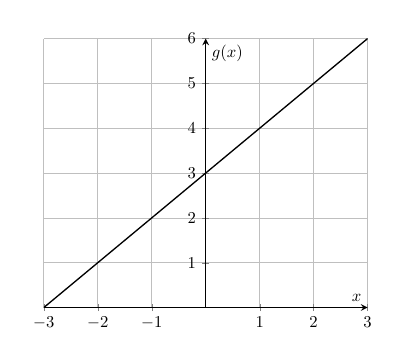
\begin{tikzpicture}[scale=0.6]
\begin{axis}[ xlabel = {$x$}, ylabel={$g(x)$}
,axis lines=middle
,grid, thick
,domain=-3:3
,xtick={-3,-2,...,3}
,ytick={0,1,...,6}
,no marks
,
]
\addplot[smooth,thick,color=black,] {x+3};

\end{axis}
\end{tikzpicture}
\end{center}

Compute the following values:

\begin{itemize}
\item $g(1)=\underline{\hspace{.25in}}$

\item $g(\underline{\hspace{.25in}})=2$


\item $f(\underline{\hspace{.25in}})=4$



\item $f(1)=\underline{\hspace{.25in}}$

\end{itemize}


\item Last winter, Anne measured the height of snow on her sidewalk during a blizzard. She defined the function $s(t)$, which gives the height of snow in inches $t$ hours after she started measuring.

\begin{figure}[h!]
\begin{center}
\begin{tikzpicture}[yscale=.75]
\draw [->] (-0.5,0) -- (4.5,0) node [right] {$t$};
\draw [->] (0,-0.5) -- (0,6.5) node [above] {$s(t)$};
\foreach \x in {1,2,3,4}
	\draw (\x,-.2) -- (\x,.2) node [at start, below] {\footnotesize\x};
\foreach \y in {2,4,6}
	\draw (-.2,\y) -- (.2,\y) node [at start, left] {\footnotesize\y};
\foreach \y in {1,3,5}
	\draw (-.2,\y) -- (0.2,\y);
\draw [very thick, domain=0:2, smooth, variable=\x] plot ({\x},{2*\x+2});
\draw [->, very thick, domain=2:5, smooth, variable=\x] plot ({\x},{0.5*\x-1});
\draw [fill=black] (0,2) circle [radius=3pt] (2,0) circle [radius=3pt] (4,1) circle [radius=3pt];
\draw [fill=white] (2,6) circle [radius=3pt];
\end{tikzpicture}
\end{center}
\end{figure}
\begin{itemize}
\item[(a)] Did  Anne  start  measuring  the  snow  when  the  blizzard  began?   How  do  you  know?
\vspace{.5 in}
\item[(b)] When is it reasonable to conclude that someone shoveled the snow on Anne’s sidewalk?  How do you know?
\vspace{1.5 in}
\end{itemize}

\newpage \item Consider the function $f(x)=13x+250$.
\begin{itemize}
	\item[(a)] What is the slope of a line whose graph is parallel to the graph of $f(x)$?
\vfill
	\item[(b)] What is the slope of a line whose graph is perpendicular to the graph of $f(x)$?\vfill
	\item[(c)] Find a formula for a line whose graph is perpenducular to the graph of $f(x)$ which passes through the point $(0, 100)$.\vfill

	\item[(d)] Let $g(x)=-13x-25$. Compare the magnitudes of the slopes of $g(x)$ and $f(x)$. What does this tell you about the steepness of their graphs?\vfill
	\item[(e)] Let $h(x)=-10x+150$. Compare the magnitudes of the slopes of $h(x)$ and $f(x)$. What does this tell you about the steepness of their graphs?\vfill

\end{itemize}

\item Let $P(t)$ give the yearly profit in dollars of a pizza restaurant, where $t$ is the number of years since they opened in 2003. Say the restaurant's yearly profit in 2005 was \$85,500, and the restaurant's yearly profit in 2018 was \$115,400. Find and \textbf{interpret} the average rate of change of the restaurant's yearly profit on the interval $[2,15]$. \textit{Be sure to write your answer in a complete sentence with units.}
\vspace{3in}


\newpage\item Samantha makes bracelets to sell at the local farmers' market every Saturday. Let the number of bracelets Samantha has in stock after $h$ hours of working at the farmers' market be given by $B(h)=325-25h$.
\begin{itemize}
	\item[(a)] Find and interpret the slope of $B(h)$. \textit{Be sure to write your answer in a complete sentence with units.}
\vspace{2in}
	\item[(b)] Find and interpret the vertical intercept of $B(h)$. \textit{Be sure to write your answer in a complete sentence with units.}
\vspace{2in}
	\item[(c)] Find and interpret the horizontal intercept of $B(h)$. \textit{Be sure to write your answer in a complete sentence with units.}
\vspace{2in}
\end{itemize}
\end{enumerate} 

\end{document}
